\section{Applications and Evaluation}
\label{sec:hotpot:app}

This section presents the performance evaluation of two applications and a set of microbenchmarks.
We ran all experiments on a cluster of 17 machines, each with two Intel Xeon CPU E5-2620 2.40GHz
processors, 128 GB DRAM, and one 40 Gbps Mellanox ConnectX-3 InfiniBand network adapter;
a Mellanox 40 Gbps InfiniBand switch connects all of the machines. 
All machines run the CentOS 7.1 distribution and the 3.11.1 Linux kernel.

The focus of our evaluation is to understand the performance of \dsnvm's distributed memory model,
its commit protocols, and its data persistence cost. As there is no real \nvm\ in production yet,
we use DRAM as stand-in for \nvm. A previous study~\cite{Zhang15-NVMMStudy} shows that even though
\nvm\ and DRAM can have some performance difference, the difference is small and has much lower impact
on application performance than the cost of flushing data from CPU caches to \nvm, which we have
included in \hotpot\ and can measure accurately.

\subsection{Systems in Comparison}
\label{sec:hotpot:comparesys}
We compare \hotpot\ with one in-memory file system, two \nvm-based file systems, 
one replicated \nvm-based system, and three distributed shared memory systems.
Below we briefly describe these systems in comparison.

\noindent{\textbf{Single-Node File Systems.}} 
Tmpfs is a Linux file system that stores all data in main memory and does not perform any I/Os to storage devices.
\pmfs~\cite{Dulloor14-EuroSys} is a file system designed for \nvm. 
The key difference between \pmfs\ and a conventional file system is that its implementation of
\mmap\ maps the physical \nvm\ pages directly into the applications' address spaces rather than moving them back and
forth between the file store and the buffer cache.
\pmfs\ ensures data persistence using \sfence\ and \clflush\ instructions.

\noindent{\textbf{Distributed \nvm-Based Systems}}
Octopus~\cite{Octopus} is a user-level RDMA-based distributed file system designed for \nvm.
\Octopus\ provides a set of customized file APIs including read and write,
but does not support memory-mapped I/Os or provide data reliability and availability.
%Octopus data servers access local PM without stacking a local file system layer. In Octopus,
%files are distributed to data servers in a hash-based way.

Mojim~\cite{Zhang15-Mojim} is our previous work that uses a primary-backup model to replicate \nvm\ data
over a customized IB layer.
Similar to \hotpot, \pmfs, and Octopus, Mojim maps \nvm\ pages directly into application virtual memory address spaces.
Mojim supports application reads and writes on the primary node but only reads on backup nodes. 

\noindent\textbf{Distributed Shared Memory Systems.} 
We implemented two kernel-level DSM systems, {\em \dsmxact} and {\em \dsmnoxact}, on top of the same network stack as \hotpot's.
Both of them support multiple readers and single writer (MRSW)
and use a home node for each memory page to serve remote read and to store which nodes are the current readers and writer of the page, 
similar to HLRC~\cite{Li89-ACM,HLRC}.
We open source both these DSM systems together with \hotpot.

{
\begin{figure*}[th]\normalsize
\begin{minipage}{3.2in}
\begin{center}
\begin{tabular}{ c | c | c | c | c | c }\normalsize
\normalsize Workload & \normalsize Read & \normalsize Update & \normalsize Scan & \normalsize Insert & \normalsize R\&U \\
\hline
A & 50\% & 50\% & - & - & - \\
B & 95\% & 5\% & - & - & - \\
C & 100\% & - & - & - & - \\
D & 95\% & - & - & 5\% & - \\
E & - & - & 95\% & 5\% & - \\
F & 50\% & - & - & - & 50\% \\
\end{tabular}
\end{center}
\vspace{-0.2in}
\mycaption{tbl-ycsb}{YCSB Workload Properties.}
{
The percentage of operations in each YCSB workload. 
R\&U stands for Read and Update.
}
\end{minipage}
\begin{minipage}{0.05in}
\hspace{0.05in}
\end{minipage}
\begin{minipage}{3.6in}
\begin{center}
\centerline{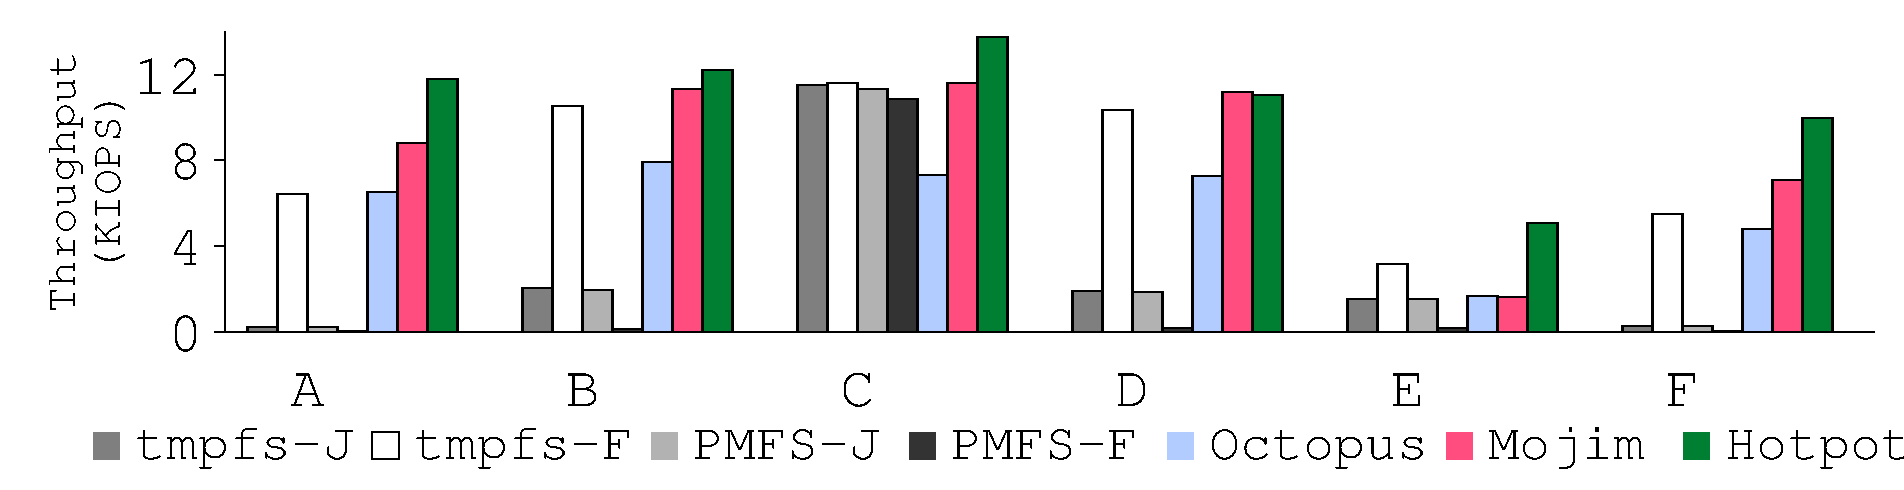
\includegraphics[width=3.8in]{Figures/g_plot_YCSB_run_throughput.pdf}}
\mycaption{fig-ycsbrun}{YCSB Workloads Throughput.}
{
}
\end{center}
\end{minipage}
\vspace{-0.2in}
\end{figure*}
}


\dsmxact\ guarantees release consistency using a transaction interface that is similar to \hotpot's \mrsw\ mode. 
Applications first call a transaction begin API to specify the data that they want to write.
Transaction begin only succeeds if no other writer is writing to any of the transaction data.
After beginning a transaction, applications can read and write to any transaction data
and use a transaction commit call to end a transaction. 
When committing a transaction, \dsmxact\ writes all updated transaction data to the home node, 
invalidates the read caches on all other nodes, 
and releases the write permission.

\dsmnoxact\ supports write (memory stores) without transactions and 
does not require applications to declare which data they want to write in advance.
On each write (memory store), \dsmnoxact\ revokes the write permission from the current writer, 
writes the current dirty data to the home node, and grants the write permission to the new writer.
Compared to \dsmxact, \dsmnoxact\ supports stronger consistency, requires less programmer efforts, 
but incurs higher performance overhead because of its more frequent writer invalidation.

Apart from the two DSM systems that we built, 
we also compare \hotpot\ with Grappa~\cite{Nelson15-ATC}, 
a recent DSM system that supports modern data-parallel applications. 
Different from traditional DSM systems and our DSM systems, Grappa moves computation to data instead of fetching data to where computation is.


\subsection{In-Memory NoSQL Database}
\label{sec:hotpot:mongodb}
MongoDB~\cite{MongoDB} is a popular distributed NoSQL database that supports several different storage engines
including its own storage engine that is based on memory-mapped files (called MMAPv1).
Applications like MongoDB can largely benefit from having a fast means to store and access persistent data. 
We ported MongoDB v2.7.0 to \hotpot\ by modifying its storage engine to keep track of all writes to the memory-mapped data file.
We then group the written memory regions belonging to the same client request into a \hotpot\ \commit\ call.
In total, porting MongoDB to \hotpot\ requires modifying 120 lines of code. 

To use the ported MongoDB, administrators can simply configure several machines to share 
a \dsnvm\ space under \hotpot\ and run ported MongoDB on each machine.
Applications on top of the ported MongoDB can issue requests to any machine, 
since all machines access the same \dsnvm\ space.
In our experiments, we ran the ported MongoDB on three \hotpot\ nodes
and set data replication degree to three.

We compare this ported MongoDB with the default MongoDB running on \tmpfs, \pmfs, and \Octopus, 
and a ported MongoDB to \Mojim\ on three nodes connected with IB.
Because \Octopus\ does not memory-mapped operations and MongoDB's storage engine is based on memory-mapped files,
MongoDB cannot directly run on \Octopus.
We run MongoDB on top of FUSE~\cite{fuse-fs}, a full-fledged user-level file system, 
which in turn runs on \Octopus.

%All these systems have three replicas of all data.
%\tmpfs, \pmfs, and \Octopus\ use MongoDB's default replication mechanism, 
For \tmpfs\ and \pmfs, we use two consistency models (called MongoDB write concerns):
the \journaled\ write concern and the \fsyncsafe\ write concern. With the \journaled\ write concern, MongoDB
logs data in a journal file and checkpoints the data in a lazy fashion. MongoDB blocks a client call until the
updated data is written to the journal file. With \fsyncsafe, MongoDB does not perform journaling. Instead, it flushes
all the dirty pages to the data file after each write operation and blocks the client call until this operation completes.
We run \Octopus\ and \Mojim\ with the \fsyncsafe\ write concern.
\Octopus, \tmpfs, and \pmfs\ provide no replication,
while \Mojim\ and \hotpot\ use their own replication mechanisms to make three replicas of all data 
(\Mojim\ uses one node as the primary node and the other two nodes as backup nodes).

\if 0
We first evaluate a simple microbenchmark that inserts key-value pairs to MongoDB. 
Each insert operation contains 10 key-value pairs, with each pair containing 100 bytes of randomly generated data.
Figure~\ref{fig-ycsbload} presents the average latency (in log scale) of key-value pair insertions. 
MongoDB on \hotpot\ outperforms the both write concerns on \pmfs.
\pmfs\ performs worse mainly because of its file system layer software overhead 
and inefficient process of making data persistent.
%uses a more efficient network layer. 
%\journaled\ write concern needs to make journal persistent
%and \fsyncsafe\ write concern makes the whole data file persistent at every write.
%This performance gain is mainly due to \hotpot's efficient replication protocol and networking stack.
\fi


{
\begin{figure*}[th]
\begin{center}
\centerline{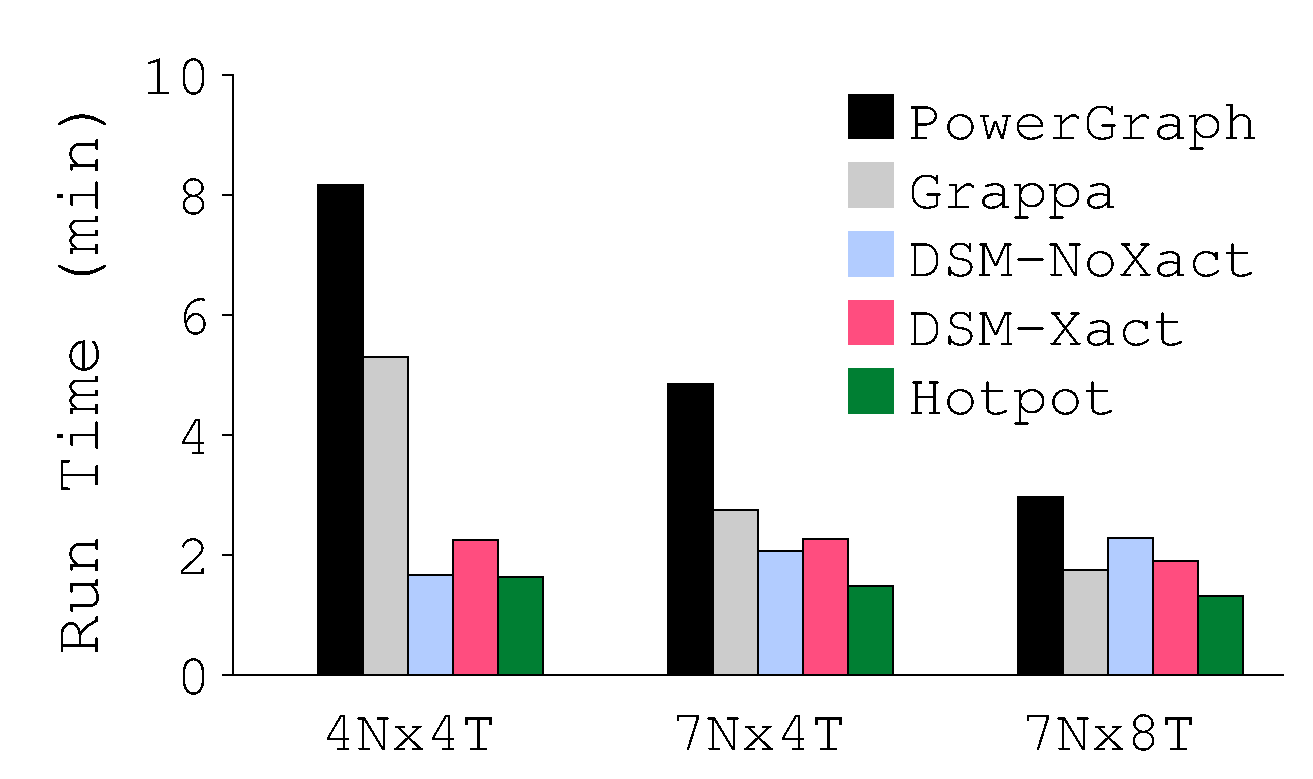
\includegraphics[width=0.6\textwidth]{hotpot/Figures/g_plot_graph_ATC_runtime.pdf}}
\caption[Pagerank Total Run Time.]
{
Pagerank Total Run Time.
N stands for total number of nodes, T stands for number of threads running on a node.
}
\label{fig-graph-runtime}
\end{center}
\end{figure*}
}
{
\begin{figure*}[th]
\begin{center}
\centerline{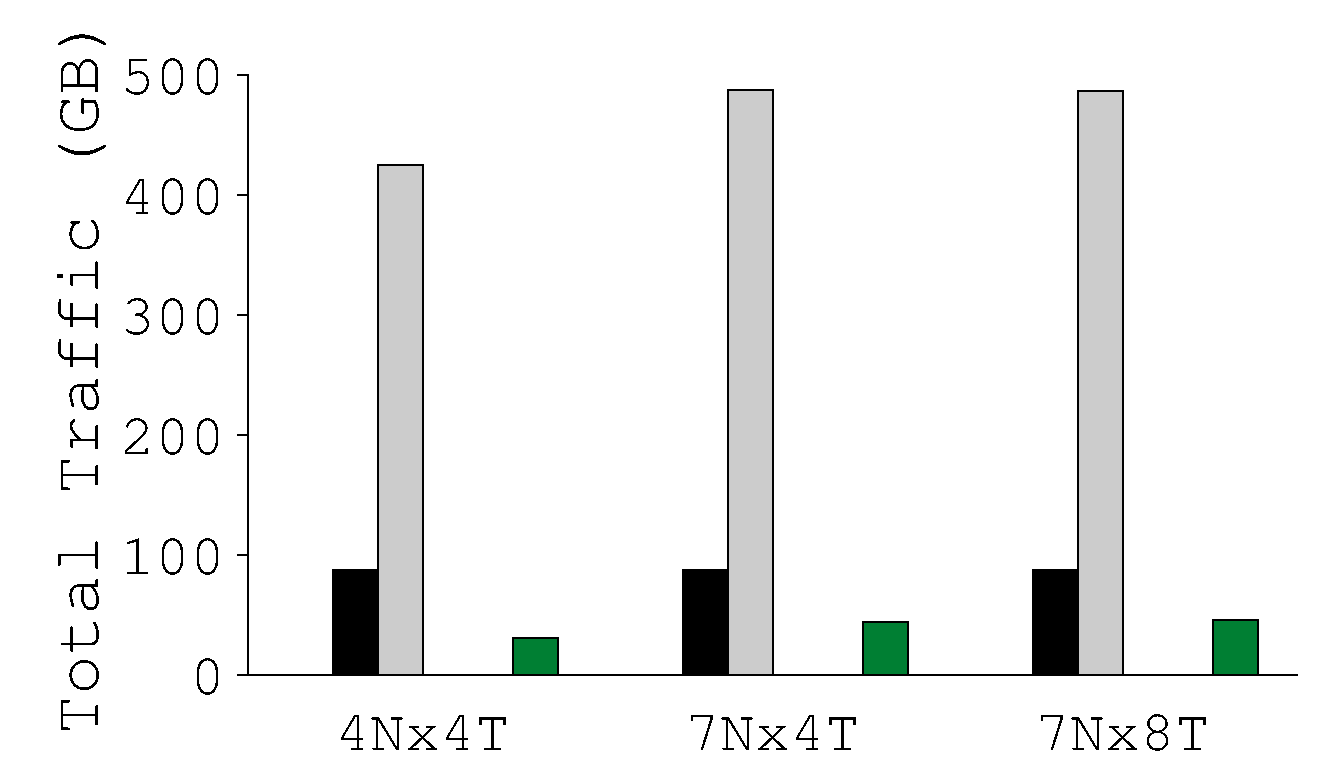
\includegraphics[width=0.6\textwidth]{hotpot/Figures/g_plot_graph_ATC_network.pdf}}
\caption[Pagerank Total Network Traffic.]
{
Pagerank Total Network Traffic.
}
\label{fig-graph-traffic}
\end{center}
\end{figure*}
}
{
\begin{figure*}[th]
\begin{center}
\centerline{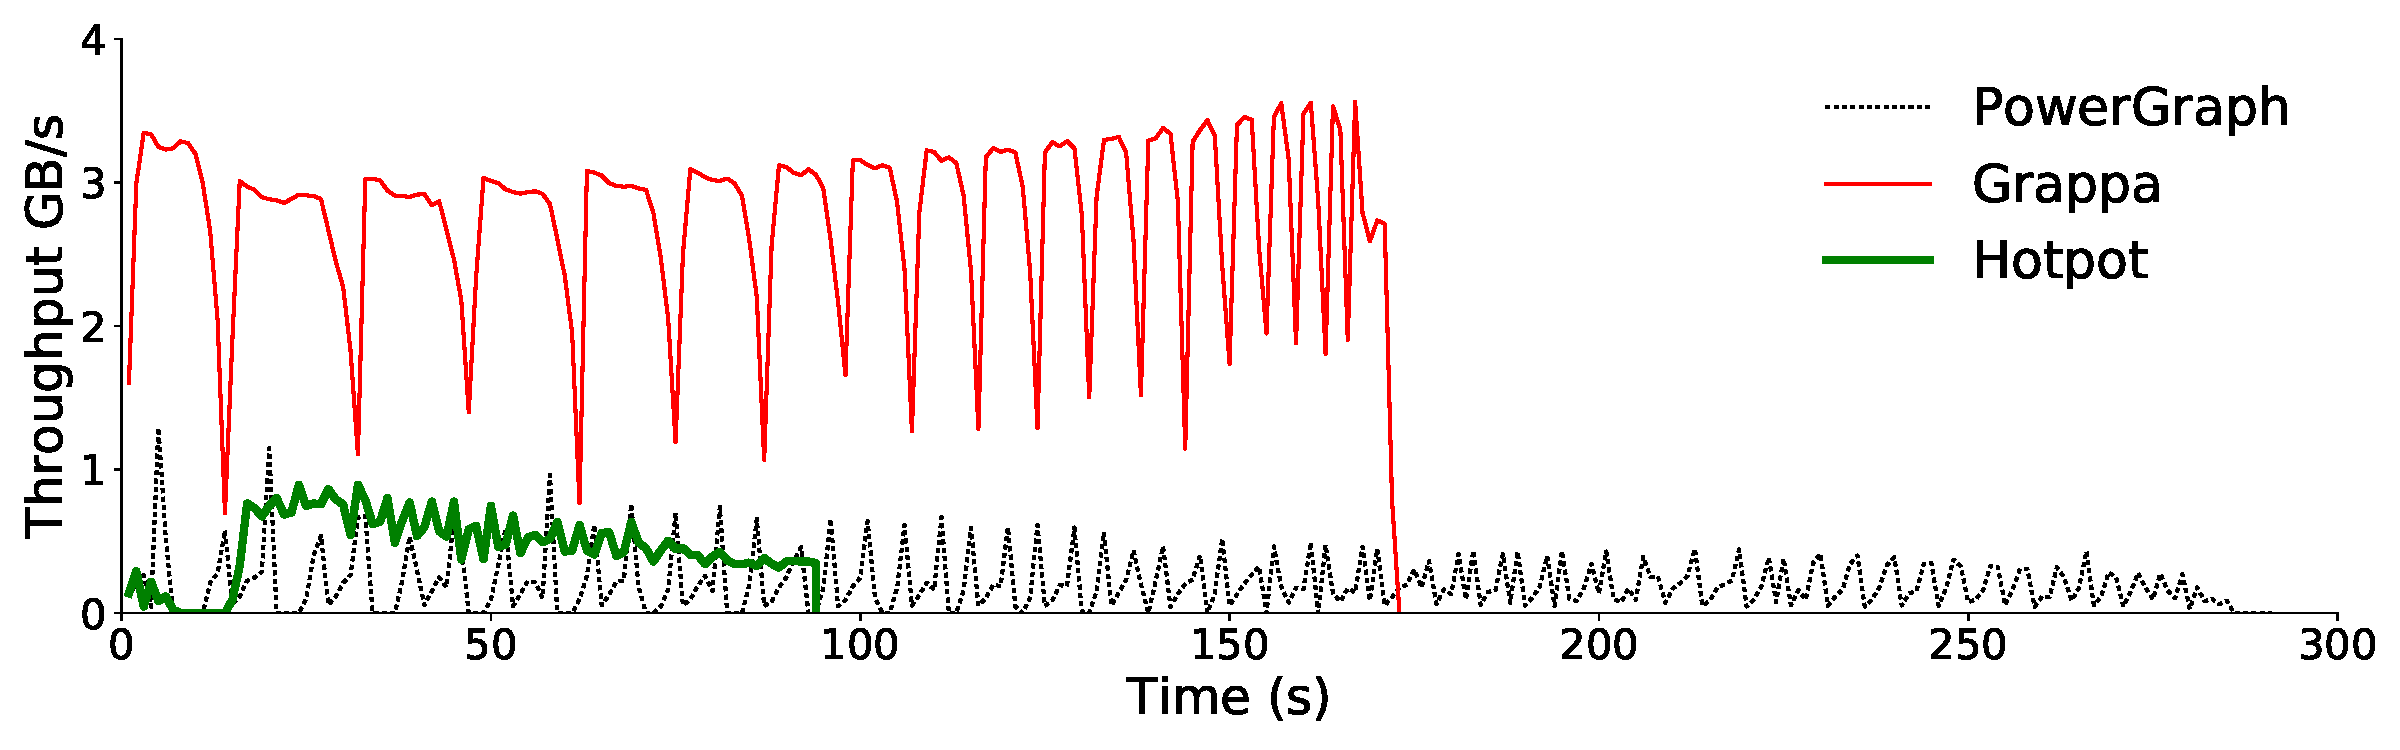
\includegraphics[width=\textwidth]{hotpot/Figures/g_plot_combined_trace_timewindow.pdf}}
\caption[Pagerank Network Traffic Over Time.]{Pagerank Network Traffic Over Time.}
\label{fig-graph-timeline}
\end{center}
\end{figure*}
}


YCSB~\cite{Cooper10-CloudCom} is a key-value store benchmark 
that imitates web applications' data access models. 
Figure~\ref{tbl-ycsb} summarizes the number of different operations in the YCSB workloads.
Each workload performs 10,000 operations on a database with 100,000 1\KB\ records.
Figure~\ref{fig-ycsbrun} presents the throughput of MongoDB on \tmpfs, \pmfs, Octopus, Mojim, and \hotpot\ using YCSB workloads. 

For all workloads, \hotpot\ outperforms \tmpfs, \pmfs, \Octopus, and \Mojim\ for both the \journaled\ and the \fsyncsafe\ write concerns. 
The performance improvement is especially high for write-heavy workloads.
\pmfs\ performs worst mainly because of its inefficient process of making data persistent with default MongoDB.
The default MongoDB \fsync{}s the whole data file after each write under \fsyncsafe,
and \pmfs\ flushes all cache lines of the file to \nvm\ by performing one \clflush\ at a time.
\hotpot\ and Mojim only commit dirty data, largely improving MongoDB performance over \pmfs.
Compared to \tmpfs\ and \pmfs\ under \journaled, \hotpot\ and Mojim use their own mechanisms to 
ensure data reliability and avoid the performance cost of journaling.
Moreover, \hotpot\ and Mojim make three persistent replica for all data, while \pmfs\ makes only one.
Tmpfs is slower than \hotpot\ even though \tmpfs\ does not make any data persistent, 
because MongoDB's slower replication mechanism on IPoIB.
\hotpot's network layer is significantly better than IPoIB~\cite{lite-sosp17}.

\Octopus\ performs worse than \hotpot\ and \Mojim\ because it incurs significant overhead of additional {\em indirection layers}:
each memory operation within the memory-mapped file goes through the FUSE file system and then through \Octopus.
\hotpot\ and \Mojim\ both support native memory instructions and incurs no indirection overhead.
Finally, even though Mojim's replication protocol is simpler and faster than \hotpot's,
\hotpot\ outperforms Mojim because Mojim only supports write on one node while \hotpot\ supports write on all nodes.

\subsection{Distributed (Persistent) Graph}
Graph processing is an increasingly important type of applications in modern 
datacenters~\cite{Gonzalez12-OSDI,Gonzalez14-OSDI,Kyrola12-OSDI,Low10-UAI,Low12-VLDB,Malewicz10-SIGMOD}.
Most graph systems require large memory to run big graphs.
Running graph algorithms on \nvm\ not only enables them to exploit the big memory space the high-density \nvm\ provides,
but can also enable graph algorithms to stop and resume in the middle of a long run.

We implemented a distributed graph processing engine on top of \hotpot\ based on the PowerGraph design~\cite{Gonzalez12-OSDI}.
It stores graphs with vertex-centric representation in \dsnvm\ with random order of vertices
and distributes graph processing load to multiple threads across all \hotpot\ nodes.
Each thread performs graph algorithms on a set of vertices in three steps: gather, apply, and scatter, 
with the optimization of delta caching~\cite{Gonzalez12-OSDI}.
After each step, we perform a global synchronization with \barrier\ and only start the next step when all threads have finished the last step.
At the scatter step, the graph engine uses \hotpot's \mrsw\ \commitxact\ to make local changes of the scatter values 
visible to all nodes in the system. We implemented the \hotpot\ graph engine with only around 700 lines of code.
Similarly, we implemented two distributed graph engines on top of \dsmxact\ and \dsmnoxact;
these engines differ from \hotpot's graph engine only in the way they perform data write and commit.

We compare \hotpot's graph engine with \dsmxact, \dsmnoxact, PowerGraph, and Grappa~\cite{Nelson15-ATC} with two real datasets,
Twitter (41\,M vertices, 1\,B directed edges)~\cite{Kwak10-WWW} and LiveJournal (4\,M vertices, 34.7\,M undirected edges)~\cite{snapnets}.
For space reason, we only present the results of the Twitter graph, but the results of LiveJournal are similar.
Figure~\ref{fig-graph-runtime} shows the total run time of the PageRank~\cite{PageRank} algorithm with
\hotpot, \dsmxact, \dsmnoxact, PowerGraph, and Grappa under three system settings:
four nodes each running four graph threads, seven nodes each running four threads, and seven nodes each running eight threads.

\hotpot\ outperforms PowerGraph by 2.3\x\ to 5\x\ and Grappa by 1.3\x\ to 3.2\x.
In addition, \hotpot\ makes all intermediate results of graph persistent for fast restart. 
A major reason why \hotpot\ outperforms PowerGraph and Grappa even when \hotpot\
requires data persistence and replication is \hotpot's network stack.
Compare to the IPoIB used in PowerGraph and Grappa's own network stack,
\hotpot's RDMA stack is more efficient.

Our implementation of \dsmxact\ and \dsmnoxact\ use the same network stack as \hotpot,
but \hotpot\ still outperforms \dsmnoxact\.
\dsmnoxact\ ensures cache coherence on every write and thus incurs much higher performance overhead than \hotpot\ and \dsmxact.

To further understand the performance differences, we traced the network traffic of these three systems.
Figure~\ref{fig-graph-traffic} plots the total amount of traffic %in the PageRank run for PowerGraph, Grappa, and \hotpot. 
and Figure~\ref{fig-graph-timeline} plots a detailed trace of network activity of the 7Nx4T setting.
\hotpot\ sends less total traffic and achieves higher bandwidth than PowerGraph and Grappa.
